\documentclass[11pt]{amsart}
\usepackage[margin=1.1in]{geometry}
\usepackage{amsmath,amssymb,amsthm}
\usepackage{graphicx}
\usepackage{booktabs}
\usepackage{xcolor}
\usepackage[colorlinks=true,linkcolor=blue!60!black,citecolor=blue!60!black,urlcolor=blue!60!black]{hyperref}
\usepackage[capitalize,nameinlink]{cleveref}

\newtheorem{theorem}{Theorem}[section]
\newtheorem{proposition}[theorem]{Proposition}
\newtheorem{lemma}[theorem]{Lemma}
\newtheorem{corollary}[theorem]{Corollary}
\theoremstyle{definition}
\newtheorem{definition}[theorem]{Definition}
\newtheorem{remark}[theorem]{Remark}
\newtheorem{question}[theorem]{Question}

\newcommand{\R}{\mathbb{R}}
\newcommand{\Z}{\mathbb{Z}}
\newcommand{\N}{\mathbb{N}}
\newcommand{\E}{\mathbb{E}}
\newcommand{\Prob}{\mathbb{P}}
\newcommand{\Law}{\mathcal{L}}
\newcommand{\Nor}{\mathcal{N}}
\newcommand{\Cond}{\mathcal{C}}
\newcommand{\Ind}{\mathbf{1}}
\DeclareMathOperator{\Var}{Var}
\DeclareMathOperator{\Cov}{Cov}
\DeclareMathOperator{\supp}{supp}

\title[Non-Gaussian degree counts in conditioned Galton--Watson trees]{Non-Gaussian fluctuations of degree counts in conditioned Galton--Watson trees}
\author{Yitzchak Shmalo}
\address{Einstein Institute of Mathematics, The Hebrew University of Jerusalem, Jerusalem, Israel}
\email{yitzchak.shmalo@gmail.com}
\date{\today}

\begin{document}

\begin{abstract}
Let $T_n$ be a Galton--Watson tree conditioned to have $n$ vertices and let $N_A(T_n)$ be the number of its vertices whose outdegree lies in $A$. Th\'evenin conjectured that $(N_A(T_n)-n\mu_A)/\sqrt n$ is asymptotically normal with variance $\mu_A(1-\mu_A)$ for every subcritical offspring law $\mu$ without exponential moment and every critical law with infinite variance. We show that the conjecture fails for an explicit subcritical law with finite third moment and for a critical law with infinite variance: along a sequence of sizes the normalised number of vertices of outdegree one converges to an equal mixture of two Gaussian laws with different means. For the subcritical law the same holds for every set $A$ with $0<\mu_A<1$, in particular for the number of leaves. We also prove a joint central limit theorem for the box counts of balls-in-boxes models when the limiting density of balls is below the critical density, and at the critical density under a second moment condition when the number of balls exceeds its critical value by at most $O(\sqrt n)$. These results answer parts of Problems 21.2--21.4 in Janson's survey of simply generated trees.
\end{abstract}

\maketitle

\section{Introduction}

Let $\mu=(\mu_k)_{k\ge0}$ be a probability distribution on the non-negative integers with $\mu_0>0$ and $\mu_0+\mu_1<1$, and let $\xi$ be a random variable with law $\mu$. A Galton--Watson tree with offspring law $\mu$ is the family tree of a branching process in which every individual has an independent number of children distributed as $\xi$; we regard it as a rooted plane tree. Let $T_n$ denote this tree conditioned to have exactly $n$ vertices, which is defined for every $n$ for which the unconditioned tree has $n$ vertices with positive probability. For $A\subset\Z_{\ge0}$ let $N_A(T_n)$ be the number of vertices of $T_n$ whose outdegree (number of children) belongs to $A$, and write $\mu_A=\sum_{k\in A}\mu_k$ and $N_k=N_{\{k\}}$. The law $\mu$ is critical if $\E\xi=1$ and subcritical if $\E\xi<1$.

The law of large numbers $N_A(T_n)/n\to\mu_A$ holds under no assumption beyond the ones above (Janson \cite[Theorem 7.11]{Janson12}). In the critical case with finite variance, Kolchin \cite[Theorem 2.3.1]{Kolchin} proved that $N_d(T_n)$ is asymptotically normal with variance $\mu_d\big(1-\mu_d-(d-1)^2\mu_d/\sigma^2\big)$, where $\sigma^2=\Var\xi$; see \cite[(21.5)--(21.7)]{Janson12} for this and for the joint version under a third moment, and Janson \cite[Example 2.2]{Janson16} for the joint version under finite variance alone. Th\'evenin \cite{Thevenin} proves functional versions of such results, and also treats a subcritical case. In the subcritical case the conditioned tree exhibits condensation: one vertex has outdegree close to $(1-\E\xi)n$, and the rest of the tree looks like a forest of small subcritical trees (Jonsson and Stef\'ansson \cite{JS}, Janson \cite[Section 19]{Janson12}, Kortchemski \cite{Kortchemski}, Abraham and Delmas \cite{AD}). Th\'evenin's Theorem 6.7 in \cite{Thevenin} states that if $\mu$ is subcritical with $\mu_k\sim ck^{-\beta}$ for some $c>0$ and $\beta>2$, then for finite sets $A_1,\dots,A_p$ the vector
\[
\Big(\frac{N_{A_i}(T_n)-n\mu_{A_i}}{\sqrt n}\Big)_{1\le i\le p}
\]
converges in distribution to a centred Gaussian vector with covariances $\mu_{A_i\cap A_j}-\mu_{A_i}\mu_{A_j}$. The section closes with the following conjecture, which we quote in full:

\begin{quote}
``We believe that these conclusions should hold for any $\mu$ critical with infinite variance, as well as for $\mu$ subcritical with no exponential moment. In particular, we should get, for any $A\subset\Z_+$,
\[
\frac{N_A(T_n)-n\mu_A}{\sqrt n}\ \xrightarrow{d}\ \Nor\big(0,\mu_A(1-\mu_A)\big).\text{''}
\]
\end{quote}

The conjecture is preceded in \cite{Thevenin} by the observation that its conclusions are already known for critical $\mu$ in the domain of attraction of a stable law and for subcritical power laws; what is at issue is the step beyond those classes. Closely related questions are Problems 21.2--21.4 of Janson's survey \cite{Janson12}. Problem 21.2 asks whether the refinements of the degree-count central limit theorem that are proved under extra moment conditions hold for critical laws with finite variance alone, whether the results extend to critical laws with infinite variance, and what happens in the condensation case $0\le\nu<1$, which contains every subcritical law without exponential moment ($\nu$ is recalled before \cref{thm:bb}); Problem 21.3 asks for the same results for the box counts of balls-in-boxes models, and Problem 21.4 for the fringe subtree counts, that is, the numbers of vertices whose subtree is a given tree.

We show that the conjecture fails for an explicit subcritical law and for a critical law with infinite variance. In both examples the normalised number of vertices of outdegree one converges along a sequence of sizes to an equal mixture of two Gaussian laws with means of opposite sign, and for the subcritical example the same is true for $N_A$ with any $A$ such that $0<\mu_A<1$, in particular for the number of leaves.

\begin{theorem}\label{thm:sub}
Let $q=1/4$, $n_1=256$, $n_{r+1}=n_r^4$, $d_0=3/4$, and for $r\ge1$
\begin{equation}\label{eq:law}
H_r=d_{r-1}n_r,\qquad L_r^{\pm}=H_r\pm\sqrt{n_r},\qquad p_r=n_r^{-4},\qquad d_r=d_{r-1}\big(1-2n_r^{-3}\big).
\end{equation}
Let $\pi$ be the law on $\Z_{\ge0}$ with $\pi_1=q$, $\pi_{L_r^-}=\pi_{L_r^+}=p_r$ for every $r\ge1$, $\pi_0=3/4-2\sum_{r\ge1}p_r$, and no other mass, and let $\xi$ have law $\pi$. Then:
\begin{enumerate}
\item[(i)] $\pi$ is a probability law with $\pi_0>1/2$; $H_r$ and $L_r^\pm$ are positive integers; $\nu=\E\xi\in(1/4,5/16)$; $\E\xi^h<\infty$ for $0<h<4$ and $\E\xi^h=\infty$ for $h\ge4$; $\E e^{\theta\xi}=\infty$ for every $\theta>0$; and $T_n$ is defined for every $n\ge1$.
\item[(ii)] With $\sigma^2=\Var\xi$, $\gamma=q(1-\nu)$,
\begin{equation}\label{eq:consts}
a_*=\frac{\gamma}{\sigma^2},\qquad v_*=q(1-q)-\frac{\gamma^2}{\sigma^2}>0,
\end{equation}
one has, as $r\to\infty$,
\begin{equation}\label{eq:sublimit}
\frac{N_1(T_{n_r})-n_rq}{\sqrt{n_r}}\ \xrightarrow{d}\ \tfrac12\Nor(-a_*,v_*)+\tfrac12\Nor(a_*,v_*).
\end{equation}
\item[(iii)] Along the same sequence, with probability tending to one, $T_{n_r}$ has exactly one vertex of outdegree larger than $n_r^{1/4}$; its outdegree is $L_r^+$ or $L_r^-$, each with probability tending to $1/2$.
\end{enumerate}
Numerically, $a_*=0.999908\ldots$ and $v_*=1.72838\ldots\times10^{-5}$.
\end{theorem}

The right side of \eqref{eq:sublimit} has characteristic function $e^{-v_*s^2/2}\cos(a_*s)$, which vanishes at $s=\pi/(2a_*)$, while the characteristic function of a Gaussian law never vanishes. So the sequence $(N_1(T_n)-nq)/\sqrt n$ does not converge in distribution to $\Nor(0,q(1-q))$, nor to any Gaussian law. More concretely, since $a_*$ is close to $1$ and $v_*$ is small, $N_1(T_{n_r})$ lies within $0.02\sqrt{n_r}$ of one of the two values $n_r/4\pm\sqrt{n_r}$ with probability tending to a limit above $1-2\times10^{-6}$, whereas the conjectured Gaussian limit would place it within $0.4\sqrt{n_r}$ of $n_r/4$ with probability about $0.64$.

\begin{theorem}\label{thm:crit}
There is a probability law $\pi$ on $\Z_{\ge0}$ with $\pi_1=1/4$, $\pi_2=1/8$, $\pi_0>1/2$, $\E\xi=1$ and $\E\xi^\alpha=\infty$ for every $\alpha>1$, where $\xi$ has law $\pi$, and a sequence $n_r\to\infty$ such that
\begin{equation}\label{eq:critlimit}
\frac{N_1(T_{n_r})-n_r/4}{\sqrt{n_r}}\ \xrightarrow{d}\ \tfrac12\Nor(-1,3/16)+\tfrac12\Nor(1,3/16).
\end{equation}
The law is critical with infinite variance and no exponential moment, its support has span one, and $T_n$ is defined for every $n\ge1$.
\end{theorem}

The variance $3/16=\pi_1(1-\pi_1)$ of each component is exactly the one predicted by the conjecture; it is the means that are wrong. The law of \cref{thm:crit} is in the domain of attraction of no stable law, so it lies outside the class for which the conclusion was already known.

The mechanism is the same in both theorems. Let $\xi_1,\dots,\xi_n$ be independent with law $\pi$. By the cycle lemma the outdegrees of $T_n$, as a multiset, have the law of $(\xi_1,\dots,\xi_n)$ conditioned on $\sum_i\xi_i=n-1$. For the laws of \cref{thm:sub,thm:crit} and $n=n_r$, the conditioning is achieved, with probability tending to one, by exactly one coordinate taking one of the two values $L_r^\pm$, which lie $2\sqrt{n_r}$ apart, and by the other coordinates taking small values. The two possibilities are equally likely in the limit, because the local limit theorem gives the same probability to the two corresponding values of the sum of the small coordinates. Given the value of the large coordinate, the number of coordinates equal to one is the count of ones among independent small variables conditioned on their sum, and its fluctuations are Gaussian with a mean that depends on which of the two values was taken. The two conditional means differ by $2a_*\sqrt{n_r}$, and the mixture is not Gaussian.

In Th\'evenin's theorem the law of the large outdegree is spread over a window of width of order $\sqrt n$ with slowly varying weights $\mu_k\sim ck^{-\beta}$, so conditioning on it does not constrain the sum of the small coordinates, and the count of ones keeps its full variance $\mu_A(1-\mu_A)$. This is the step on which the proof of Theorem 6.7 of \cite{Thevenin} rests: for a subexponential law, the outdegrees other than the largest are asymptotically independent with law $\mu$ (Armend\'ariz and Loulakis \cite{AL}; see also \cite[Section 19]{Janson12}). For the laws below that description fails, because the largest outdegree can absorb only two values and the others remain conditioned on their sum. The counterexamples are lacunary: the offspring law places its mass above $1$ on a sparse set of integers, so that at the sizes $n_r$ the large outdegree can only take two values. Theorem 6.7 of \cite{Thevenin} is not affected. The examples show that the conjecture needs a regularity assumption on the tail of $\mu$, and \cref{sec:remarks} formulates the version that the argument suggests.

The mechanism does not depend on the set $A$. Given the sign of the large coordinate, every count $N_A$ is a sum of a bounded function of the small coordinates conditioned on their sum, and its conditional mean moves with the sign unless $\Ind_A(\xi)$ is uncorrelated with $\xi$. For the subcritical law this gives the following.

\begin{corollary}\label{cor:sub}
Let $\pi$, $\xi$, $\nu$, $\sigma^2$ and $(n_r)$ be as in \cref{thm:sub}, and let $A\subset\Z_{\ge0}$ with $0<\pi_A<1$. Put
\[
\gamma_A=\Cov\big(\Ind_A(\xi),\xi\big),\qquad a_A=\frac{\gamma_A}{\sigma^2},\qquad v_A=\pi_A(1-\pi_A)-\frac{\gamma_A^2}{\sigma^2}.
\]
Then $a_A\ne0$, $v_A>0$, and, as $r\to\infty$,
\[
\frac{N_A(T_{n_r})-n_r\pi_A}{\sqrt{n_r}}\ \xrightarrow{d}\ \tfrac12\Nor(-a_A,v_A)+\tfrac12\Nor(a_A,v_A).
\]
In particular the limit is not Gaussian.
\end{corollary}

For $A=\{1\}$ this is \cref{thm:sub}(ii), with $a_{\{1\}}=a_*$ and $v_{\{1\}}=v_*$. For the leaves, $A=\{0\}$, one has $\gamma_{\{0\}}=-\nu\pi_0$, $a_{\{0\}}=-0.999908\ldots$ and $v_{\{0\}}=1.71054\ldots\times10^{-5}$, so that, as for the vertices of outdegree one, the number of leaves of $T_{n_r}$ concentrates near the two values $n_r\pi_0\pm\sqrt{n_r}$. For this law the conjecture thus fails for every $A$ with $0<\pi_A<1$; when $\pi_A\in\{0,1\}$ both sides are the point mass at $0$.

The tree is a special case of the balls-in-boxes model of \cite[Section 11]{Janson12}, and the local limit theorem behind \cref{thm:sub,thm:crit} also gives the positive side of the picture in that generality. Let $w=(w_k)_{k\ge0}$ be non-negative weights with $w_0>0$ and span one, that is, $\gcd\{k:w_k>0\}=1$. For integers $m\ge0$ and $n\ge1$ the random allocation $B_{m,n}=(y_1,\dots,y_n)$ is the random vector of non-negative integers with $\sum_iy_i=m$ whose probabilities are proportional to $\prod_iw_{y_i}$; it is defined when some such vector has positive weight. Let $N_A(B_{m,n})=\#\{i\le n:y_i\in A\}$ be the number of boxes whose number of balls lies in $A$. Let $\Phi(t)=\sum_kw_kt^k$, let $\rho\in[0,\infty]$ be its radius of convergence, and for $t>0$ with $\Phi(t)<\infty$ let $\pi^t$ be the law with $\pi^t_k=w_kt^k/\Phi(t)$. For $0<t<\rho$ the mean of $\pi^t$ is $\Psi(t)=t\Phi'(t)/\Phi(t)$; it increases continuously and strictly, since $\Psi'(t)=\Var(\pi^t)/t>0$, and tends to $0$ as $t\to0$. Let $\nu=\lim_{t\uparrow\rho}\Psi(t)\in(0,\infty]$ if $\rho>0$, and $\nu=0$ if $\rho=0$. If $0<\rho<\infty$ and $\nu<\infty$, then $\Phi(\rho)<\infty$ \cite[Lemma 3.1]{Janson12} and $\pi^\rho$ has mean $\nu$. By \cref{lem:cycle}, $N_A(T_n)$ has the law of $N_A(B_{n-1,n})$ for the weights $w=\mu$; when $\mu$ has no exponential moment, $\rho=1$, $\pi^1=\mu$ and $\nu=\E\xi$, in accordance with the notation of \cref{thm:sub}.

\begin{theorem}\label{thm:bb}
Let $w$ be as above, let $A_1,\dots,A_p\subset\Z_{\ge0}$, and let $m=m(n)$ be integers with $m/n\to\lambda\in(0,\infty)$. For $0<t\le\rho$ such that $\pi^t$ is defined and has finite variance, and $X$ with law $\pi^t$, let $\Sigma(t)$ be the $p\times p$ matrix with entries
\[
\Sigma_{jl}(t)=\pi^t(A_j\cap A_l)-\pi^t(A_j)\,\pi^t(A_l)-\frac{\gamma_j(t)\gamma_l(t)}{\Var X},\qquad\gamma_j(t)=\Cov\big(\Ind_{A_j}(X),X\big).
\]
\begin{enumerate}
\item[(a)] Suppose that $\lambda<\nu$, or that $\lambda=\nu$, $\rho<\infty$, $\Var(\pi^\rho)<\infty$ and $m<n\nu$ for all large $n$. Let $\tau\in(0,\rho]$ be given by $\Psi(\tau)=\lambda$ if $\lambda<\nu$, and $\tau=\rho$ if $\lambda=\nu$, and for large $n$ let $\tau_n\in(0,\rho)$ be given by $\Psi(\tau_n)=m/n$. Then
\[
\Big(\frac{N_{A_j}(B_{m,n})-n\,\pi^{\tau_n}(A_j)}{\sqrt n}\Big)_{j\le p}\ \xrightarrow{d}\ \Nor\big(0,\Sigma(\tau)\big).
\]
\item[(b)] Suppose that $\lambda=\nu$, $\rho<\infty$, $\Var(\pi^\rho)<\infty$ and $(m-n\nu)/\sqrt n\to a\in\R$. Then
\[
\Big(\frac{N_{A_j}(B_{m,n})-n\,\pi^{\rho}(A_j)}{\sqrt n}\Big)_{j\le p}\ \xrightarrow{d}\ \Nor\Big(\Big(\frac{a\,\gamma_j(\rho)}{\Var(\pi^\rho)}\Big)_{j\le p},\ \Sigma(\rho)\Big).
\]
\end{enumerate}
In both cases $B_{m,n}$ is defined for all large $n$.
\end{theorem}

For $A_1=\{d\}$ and $m=n-1$ the variance $\Sigma_{11}$ is Kolchin's $\pi_d\big(1-\pi_d-(d-1)^2\pi_d/\sigma^2\big)$. Part (a) with $\lambda<\nu$ is contained in Janson's conditional limit theorems \cite[Corollaries 2.1 and 2.2]{Janson01}, which also give the convergence of all moments; general conditional limit theorems of this kind go back to Steck, Holst and Kudlaev, see \cite{Janson01} and the references there. For a critical offspring law $\mu$ with finite variance and $w=\mu$, either $\nu=1$, and then $\rho=1$, or $\nu>1$ and $\tau=1<\rho$; so \cref{thm:bb} with $m=n-1$ gives the joint asymptotic normality of the degree counts centred at $n\mu_{A_j}$, by part (b) with $a=0$ in the first case and by part (a) in the second, where $n\pi^{\tau_n}(A_j)-n\mu_{A_j}=O(1)$ because $\Psi$ and $t\mapsto\pi^t(A_j)$ are smooth near $t=1$ and $\Psi'(1)>0$. This is the result of Janson \cite[Example 2.2]{Janson16}. Read as statements about $B_{n-1,n}$, \cref{thm:sub} and \cref{cor:sub} show that the conclusion of \cref{thm:bb} can fail when $\lambda>\nu$, and \cref{thm:crit} that it can fail when $\lambda=\nu$ and $\Var(\pi^\rho)=\infty$. The case $\lambda=\nu$ with $\Var(\pi^\rho)<\infty$ and $(m-n\nu)/\sqrt n\to\infty$ is not covered.

The paper is organised as follows. \Cref{sec:prelim} records the cycle lemma and a conditional local limit theorem for triangular arrays, proved by Fourier inversion. \Cref{sec:sub} proves \cref{thm:sub} and \cref{cor:sub}, \cref{sec:crit} proves \cref{thm:crit}, and \cref{sec:bb} proves \cref{thm:bb}. \Cref{sec:num} reports exact computations for the law of \cref{thm:sub} at $n=256$ and $n=2^{32}$, for $N_1(T_n)$ and for the number of leaves, and for the first stage of the construction of \cref{thm:crit}. The arithmetic facts used in the constructions (the atoms of the first two stages, the bounds on $d_r$ and on the rare mass, the exclusion of a second large coordinate, the exact centering identity, the Bernstein exponent, the mean increments of the critical law and its first-stage atoms) are proved in Lean~4 with Mathlib; the file and its build log are in the repository named at the end.

\section{Preliminaries}\label{sec:prelim}

\subsection{Degree counts and conditioned sums}

Let $\pi$ be an offspring law with $\pi_0>0$. A rooted plane tree with $n$ vertices is determined by the sequence $(k_1,\dots,k_n)$ of outdegrees of its vertices in depth-first order, and a sequence of non-negative integers arises in this way if and only if $\sum_{i\le n}k_i=n-1$ and $\sum_{i\le j}(k_i-1)\ge0$ for every $j<n$. The Galton--Watson measure gives the tree the weight $\prod_i\pi_{k_i}$.

\begin{lemma}[cycle lemma]\label{lem:cycle}
Let $\xi_1,\dots,\xi_n$ be independent with law $\pi$ and let $\Cond_n=\{\xi_1+\dots+\xi_n=n-1\}$. If $\Prob(\Cond_n)>0$ then $T_n$ is defined, $\Prob(|T|=n)=\Prob(\Cond_n)/n$, and for every function $f$ of a multiset of $n$ non-negative integers,
\[
\E\big[f(\text{outdegrees of }T_n)\big]=\E\big[f(\xi_1,\dots,\xi_n)\,\big|\,\Cond_n\big].
\]
In particular $N_A(T_n)$ has the law of $\#\{i\le n:\xi_i\in A\}$ given $\Cond_n$.
\end{lemma}

\begin{proof}
This is the classical observation of Dvoretzky and Motzkin \cite{DM}; see \cite[Section 15]{Janson12} or \cite[Section 6.1]{Pitman}. If $(x_1,\dots,x_n)$ are non-negative integers with $\sum_i x_i=n-1$, then exactly one of the $n$ cyclic rotations of the sequence satisfies the partial-sum condition, and the $n$ rotations are distinct because a proper period $d$ of the sequence would make $\sum_i(x_i-1)=-1$ divisible by $n/d\ge2$. The weight $\prod_i\pi_{x_i}$ is invariant under rotation, so the map that sends a sequence to its unique admissible rotation pushes the law of $(\xi_1,\dots,\xi_n)$ restricted to $\Cond_n$ forward to $n$ times the Galton--Watson weight of the corresponding tree. Multisets of outdegrees are rotation invariant.
\end{proof}

If $\pi_1>0$ then $\Prob(\Cond_n)\ge\pi_1^{n-1}\pi_0>0$ for every $n$, so $T_n$ is defined for all $n\ge1$; this covers both laws of the paper.

\subsection{A conditional local limit theorem}

Let $(X_r)_{r\ge1}$ be a sequence of random variables with values in $\Z_{\ge0}$, let $N_r\to\infty$ be integers, and let $f:\Z_{\ge0}\to\R$ be bounded. For each $r$ let $X_{r,1},\dots,X_{r,N_r}$ be independent copies of $X_r$ and put
\[
S_r=\sum_{i\le N_r}X_{r,i},\qquad B_r=\sum_{i\le N_r}f(X_{r,i}).
\]
Write $\mu_r=\E X_r$, $q_r=\E f(X_r)$. For $f=\Ind_A$, $B_r$ is the number of $i\le N_r$ with $X_{r,i}\in A$.

\begin{lemma}\label{lem:llt}
Assume that $X_r\to X$ in distribution, that $(X_r^2)_r$ is uniformly integrable, and that there are a finite set $F\subset\Z_{\ge0}$ whose differences have greatest common divisor one and a constant $c>0$ such that $\Prob(X_r=x)\ge c$ for every $x\in F$ and all large $r$. Put $\mu=\E X$, $\sigma^2=\Var X$, $b=\Var f(X)$ and $\gamma=\Cov(f(X),X)$. Then $\sigma^2>0$. Let $k_r$ be integers with $(k_r-N_r\mu_r)/\sqrt{N_r}\to a\in\R$. Then
\begin{equation}\label{eq:llt1}
\sqrt{N_r}\,\Prob(S_r=k_r)\longrightarrow\frac{e^{-a^2/(2\sigma^2)}}{\sqrt{2\pi\sigma^2}},
\end{equation}
and the conditional law of $(B_r-N_rq_r)/\sqrt{N_r}$ given $S_r=k_r$ converges to
\begin{equation}\label{eq:llt2}
\Nor\Big(\frac{\gamma a}{\sigma^2},\ b-\frac{\gamma^2}{\sigma^2}\Big).
\end{equation}
The variance in \eqref{eq:llt2} is positive unless $f(X)$ is almost surely an affine function of $X$.
\end{lemma}

\begin{proof}
The set $F$ has at least two elements and $\Prob(X=x)=\lim_r\Prob(X_r=x)\ge c$ for $x\in F$, so $\sigma^2>0$. Write $N=N_r$, $Y_r=f(X_r)$, $\|f\|=\sup_x|f(x)|$, and fix $s\in\R$. Since $S_r$ is integer valued, Fourier inversion gives
\begin{equation}\label{eq:inv}
\E\Big[e^{is(B_r-Nq_r)/\sqrt N};\,S_r=k_r\Big]
=\frac1{2\pi}\int_{-\pi}^{\pi}e^{-it(k_r-N\mu_r)}\,\phi_r(t,s)^N\,dt,
\end{equation}
where $\phi_r(t,s)=\E\,e^{it(X_r-\mu_r)+is(Y_r-q_r)/\sqrt N}$.
Substitute $t=v/\sqrt N$ and multiply by $\sqrt N$; the right side becomes $\frac1{2\pi}\int_{|v|\le\pi\sqrt N}e^{-iv(k_r-N\mu_r)/\sqrt N}\phi_r(v/\sqrt N,s)^N\,dv$.

\emph{Pointwise limit.} Put $W_r=v(X_r-\mu_r)+s(Y_r-q_r)$. Then $\E W_r=0$, and $\E W_r^2\to v^2\sigma^2+2vs\gamma+s^2b$: every function on the integers is continuous, so $(X_r,Y_r)\to(X,f(X))$ in distribution, and $X_r^2$, $X_rY_r$ and $Y_r^2$ are uniformly integrable because $|Y_r|\le\|f\|$, so the first and second moments of $(X_r,Y_r)$ converge. The family $(W_r^2)_r$ is uniformly integrable, so $\E e^{iW_r/\sqrt N}=1-\E W_r^2/(2N)+o(1/N)$: the second-order remainder of $e^{iw}$ at $w=W_r/\sqrt N$ is at most $\min(|w|^3/6,w^2)$, so $N$ times its expectation is at most $K\,\E W_r^2/(6\sqrt N)+\E[W_r^2;|W_r|>K]$, and one lets $K\to\infty$ after $N$. Hence $\phi_r(v/\sqrt N,s)^N\to\exp\{-\tfrac12(\sigma^2v^2+2\gamma vs+bs^2)\}$, and $e^{-iv(k_r-N\mu_r)/\sqrt N}\to e^{-iva}$.

\emph{Domination.} Let $(X_r',Y_r')$ be an independent copy of $(X_r,Y_r)$, and put $\alpha=t(X_r-X_r')$ and $\beta=s(Y_r-Y_r')/\sqrt N$. Since $e^{i(\alpha+\beta)}-1=(e^{i\alpha}-1)+e^{i\alpha}(e^{i\beta}-1)$, $|z|^2\le2|z+z'|^2+2|z'|^2$ and $|e^{ix}-1|^2=2(1-\cos x)$, we have $1-\cos(\alpha+\beta)\ge\frac12(1-\cos\alpha)-(1-\cos\beta)$, and therefore
\[
1-|\phi_r(t,s)|^2=\E\big[1-\cos(\alpha+\beta)\big]\ge\tfrac12\E[1-\cos\alpha]-\tfrac12\E\beta^2\ge\tfrac12\E[1-\cos\alpha]-\frac{2s^2\|f\|^2}N.
\]
Keeping in $\E[1-\cos\alpha]$ only the pairs of values in $F$ gives, for large $r$, $\E[1-\cos\alpha]\ge c^2g(t)$ with $g(t)=\sum_{x,y\in F}\big(1-\cos(t(x-y))\big)$. The function $g$ is continuous and non-negative, and on $[-\pi,\pi]$ it vanishes only at $0$: if $t(x-y)\in2\pi\Z$ for all $x,y\in F$, then $t\in2\pi\Z$, because $1$ is an integer combination of the differences $x-y$. Since $g(t)/t^2\to\frac12\sum_{x,y\in F}(x-y)^2>0$ as $t\to0$, there is $\kappa>0$ with $g(t)\ge\kappa t^2$ for $|t|\le\pi$. Using $|\phi|^2\le\exp\{-(1-|\phi|^2)\}$, we get for $|t|\le\pi$ and large $r$
\[
|\phi_r(t,s)|^N\le\exp\Big\{-\frac N2\Big(\frac{c^2\kappa t^2}2-\frac{2s^2\|f\|^2}N\Big)\Big\}=e^{s^2\|f\|^2}e^{-c^2\kappa Nt^2/4},
\]
so after the substitution $t=v/\sqrt N$ the integrand is bounded by $e^{s^2\|f\|^2}e^{-c^2\kappa v^2/4}$, an integrable function of $v$. Dominated convergence therefore gives
\begin{multline*}
\sqrt N\,\E\Big[e^{is(B_r-Nq_r)/\sqrt N};\,S_r=k_r\Big]
\longrightarrow\frac1{2\pi}\int_\R e^{-iva}\exp\Big\{-\tfrac12(\sigma^2v^2+2\gamma vs+bs^2)\Big\}dv\\
=\frac{e^{-a^2/(2\sigma^2)}}{\sqrt{2\pi\sigma^2}}\exp\Big\{i\frac{\gamma a}{\sigma^2}s-\frac12\Big(b-\frac{\gamma^2}{\sigma^2}\Big)s^2\Big\},
\end{multline*}
by the Gaussian integral $\int e^{-\sigma^2v^2/2-v(ia+\gamma s)}dv=\sqrt{2\pi/\sigma^2}\,e^{(ia+\gamma s)^2/(2\sigma^2)}$. At $s=0$ this is \eqref{eq:llt1}; dividing by the value at $s=0$ gives the characteristic function of \eqref{eq:llt2}, which proves the convergence of the conditional laws. The variance $b-\gamma^2/\sigma^2=\Var(Y)-\Cov(Y,X)^2/\Var(X)$, $Y=f(X)$, vanishes exactly when the Cauchy--Schwarz inequality for $(Y-\E Y,X-\mu)$ is an equality, that is, when $Y-\E Y$ is almost surely a multiple of $X-\mu$.
\end{proof}

The lemma will be used in two ways: with rows $X_r$ that vary with $r$ (\cref{sec:sub,sec:bb}) and with a fixed law and $N\to\infty$ (\cref{sec:crit,sec:bb}); the second is the case $X_r=X$ for all $r$. It extends to finitely many bounded functions $f_1,\dots,f_p$ by the Cram\'er--Wold device: with $B_r^{(j)}$, $q_r^{(j)}$ and $\gamma_j$ defined from $f_j$, the conditional law of $\big((B_r^{(j)}-N_rq_r^{(j)})/\sqrt{N_r}\big)_{j\le p}$ given $S_r=k_r$ converges to the Gaussian law with means $\gamma_ja/\sigma^2$ and covariances $\Cov(f_j(X),f_l(X))-\gamma_j\gamma_l/\sigma^2$, since for $s\in\R^p$ the lemma applied to $\sum_js_jf_j$ gives the limit law of $\sum_js_j(B_r^{(j)}-N_rq_r^{(j)})/\sqrt{N_r}$.

\subsection{Bernstein's inequality}

Let $Z_1,\dots,Z_N$ be independent with $\E Z_i=0$, $|Z_i|\le M$ and $\sum_i\Var Z_i=V$. Then for $D>0$
\begin{equation}\label{eq:bernstein}
\Prob\Big(\sum_iZ_i\ge D\Big)\le\exp\Big\{-\frac{D^2}{2(V+MD/3)}\Big\}
\end{equation}
(see \cite[Theorem 2.10]{BLM}). We use it for variables $X_i-\E X_i$ with $0\le X_i\le M$, for which $|X_i-\E X_i|\le M$.

\section{The subcritical law}\label{sec:sub}

\subsection{The law and its moments}

Throughout this section $q=1/4$ and $n_r$, $d_r$, $H_r$, $L_r^\pm$, $p_r$ are as in \eqref{eq:law}, so that $n_r=2^{8\cdot4^{r-1}}$ and $\sqrt{n_r}$ is an integer. The first two stages are
\[
\begin{array}{c|c|c|c|c|c}
r & n_r & H_r & L_r^- & L_r^+ & p_r\\ \hline
1 & 2^{8} & 192 & 176 & 208 & 2^{-32}\\
2 & 2^{32} & 3\,221\,225\,088 & 3\,221\,159\,552 & 3\,221\,290\,624 & 2^{-128}
\end{array}
\]

\begin{proposition}\label{prop:law}
\begin{enumerate}
\item[(a)] $5/8<d_r\le3/4$ for all $r\ge0$, and $d_r$ decreases to a limit $d_\infty>5/8$. The numbers $H_r$ and $L_r^\pm$ are integers with $n_r/2<L_r^-<L_r^+<n_r$.
\item[(b)] $2\sum_{r\ge1}p_r<4\cdot256^{-4}$, so $\pi_0>1/2$ and $\pi$ is a probability law.
\item[(c)] $2L_r^->n_r-1$ and $L_{r+1}^->n_r$ for every $r\ge1$.
\item[(d)] $\nu=\E\xi=1-d_\infty\in(1/4,5/16)$, $\E\xi^2<1/2$, $\E\xi^h<\infty$ for $0<h<4$, $\E\xi^h=\infty$ for $h\ge4$, and $\E e^{\theta\xi}=\infty$ for every $\theta>0$.
\end{enumerate}
\end{proposition}

\begin{proof}
(a) Since $n_r\ge256$, the invariant $d_r\ge5/8+2n_{r+1}^{-3}$ propagates: if it holds for $r$ then $d_{r+1}=d_r(1-2n_{r+1}^{-3})\ge(5/8+2x)(1-2x)$ with $x=n_{r+1}^{-3}\le2^{-24}$, and $(5/8+2x)(1-2x)=5/8+\tfrac34x-4x^2\ge5/8+2x^4=5/8+2n_{r+2}^{-3}$. It holds for $r=0$ because $d_0=3/4$. Monotonicity is clear, $d_r\le d_0$, and the bound $d_\infty>11/16$ is proved in (d). Integrality: $H_1=192$; if $H_r$ is an integer then $H_{r+1}=d_rn_{r+1}=d_{r-1}(1-2n_r^{-3})n_r^4=H_rn_r^3-2H_r$ is an integer; and $\sqrt{n_r}=n_{r-1}^2$ is an integer for $r\ge2$, $\sqrt{n_1}=16$. The bounds on $L_r^\pm$ follow from $5/8<d_{r-1}\le3/4$ and $\sqrt{n_r}\le n_r/16$.

(b) $p_r=n_r^{-4}$ and $n_{r+1}=n_r^4\ge2n_r$, so $2\sum_rp_r\le2\cdot256^{-4}\sum_{j\ge0}2^{-4j}<4\cdot256^{-4}$.

(c) $2L_r^-=2d_{r-1}n_r-2\sqrt{n_r}\ge\tfrac54n_r-2\sqrt{n_r}>n_r-1$ since $\sqrt{n_r}\ge16$; and $L_{r+1}^-\ge\tfrac58n_r^4-n_r^2>n_r$.

(d) $\E\xi=q+\sum_rp_r(L_r^-+L_r^+)=q+\sum_r2p_rH_r=q+\sum_r2d_{r-1}n_r^{-3}=q+(d_0-d_\infty)=1-d_\infty$, since $d_{r-1}-d_r=2d_{r-1}n_r^{-3}$. By (a), $\nu\in(1/4,3/8)$, and more precisely $d_\infty\ge d_1-\sum_{r\ge2}2d_{r-1}n_r^{-3}\ge d_1-\tfrac32\cdot2\cdot2^{-96}>11/16$, so $\nu<5/16$. For $h>0$, $\E\xi^h=q+\sum_rp_r((L_r^-)^h+(L_r^+)^h)$; since $d_{r-1}\ge d_\infty>11/16$ and $\sqrt{n_r}\le n_r/16$, $L_r^->\tfrac58n_r$, so $(5/8)^hn_r^{h-4}\le p_r(L_r^\pm)^h\le n_r^{h-4}$; the series converges if and only if $h<4$, and for $h=2$ it is at most $2\sum_rn_r^{-2}<4\cdot256^{-2}$, so $\E\xi^2<1/2$. Finally $p_re^{\theta L_r^-}\ge n_r^{-4}e^{5\theta n_r/8}\to\infty$.
\end{proof}

The variance $\sigma^2=\E\xi^2-\nu^2$ is positive, and $\pi$ has span one because $\pi_0,\pi_1>0$. In particular $\pi$ is subcritical, has all moments of order below four, and has no exponential moment: it satisfies every hypothesis of the conjecture. The atoms of every stage are multiples of $16$, which is used nowhere in the proof but explains the lattice structure of the exact laws in \cref{sec:num}.

\subsection{The three types of the conditioning event}

Fix $r\ge2$ and write $n=n_r$. Let $\xi_1,\dots,\xi_n$ be independent with law $\pi$ and $\Cond=\{\xi_1+\dots+\xi_n=n-1\}$. On $\Cond$ every coordinate is at most $n-1$, so by \cref{prop:law}(c) no coordinate equals $L_s^\pm$ with $s>r$, and at most one coordinate equals $L_r^+$ or $L_r^-$. Put
\[
\mathcal A_r=\{0,1\}\cup\{L_s^-,L_s^+:s<r\},\qquad t_r=2\sum_{s\ge r}p_s,\qquad z_r=\pi(\mathcal A_r)=1-t_r,
\]
and let $X_r$ have the law of $\xi$ conditioned on $\xi\in\mathcal A_r$. Then $\Cond$ splits into three disjoint events: $J=0$, all coordinates in $\mathcal A_r$; $J=1$ with sign $\varepsilon\in\{+,-\}$, exactly one coordinate equal to $L_r^\varepsilon$ and the others in $\mathcal A_r$. Let $R_{r,m}$ denote the sum of $m$ independent copies of $X_r$ and let
\[
k_r^\varepsilon=n-1-L_r^\varepsilon .
\]
Counting the position of the large coordinate,
\begin{equation}\label{eq:beta}
\beta_r^\varepsilon:=\Prob(\Cond,J=1,\text{sign }\varepsilon)=n\,p_r\,z_r^{\,n-1}\,\Prob(R_{r,n-1}=k_r^\varepsilon),
\quad
\beta_r^0:=\Prob(\Cond,J=0)=z_r^{\,n}\,\Prob(R_{r,n}=n-1).
\end{equation}

The rows $X_r$ satisfy the hypotheses of \cref{lem:llt} with $f=\Ind_{\{1\}}$, $F=\{0,1\}$ and $c=1/4$. Indeed $0<t_r\le4n^{-4}$ and $z_r>3/4$ by \cref{prop:law}(b), so $X_r\to\xi$ in distribution; $\E[X_r^2;X_r>K]\le\tfrac43\E[\xi^2;\xi>K]$ gives uniform integrability; $\Prob(X_r=0)\ge1/2$ and $\Prob(X_r=1)=q/z_r\ge1/4$. The limiting constants are $\mu=\nu$, $\sigma^2=\Var\xi$, $b=q(1-q)$ and $\gamma=q(1-\nu)$. Write
\begin{equation}\label{eq:rowmeans}
u_r=q+\sum_{s<r}p_s(L_s^-+L_s^+)=1-d_{r-1},\qquad
\mu_r=\E X_r=\frac{u_r}{z_r},\qquad
q_r=\Prob(X_r=1)=\frac q{z_r},
\end{equation}
where $u_r=1-d_{r-1}$ follows from the telescoping in the proof of \cref{prop:law}(d). Then $\mu_r-u_r=u_rt_r/z_r$ and $q_r-q=qt_r/z_r$ are $O(n^{-4})$, and $\mu_r<(5/16)/(3/4)<1/2$, $\Var X_r\le\E X_r^2\le\E\xi^2/z_r<1$. Every value of $X_r$ is at most $M_r=n_{r-1}=n^{1/4}$.

\subsection{The centering and the two large coordinates}

Since $L_r^\varepsilon=d_{r-1}n+\varepsilon\sqrt n$ and $u_r=1-d_{r-1}$,
\begin{equation}\label{eq:center}
k_r^\varepsilon-(n-1)\mu_r
=(n-1)-d_{r-1}n-\varepsilon\sqrt n-(n-1)\frac{u_r}{z_r}
=-\varepsilon\sqrt n-d_{r-1}-(n-1)\frac{u_rt_r}{z_r},
\end{equation}
an exact identity (the middle expression equals $(n-1)u_r-d_{r-1}-\varepsilon\sqrt n-(n-1)u_r/z_r$ and $1/z_r-1=t_r/z_r$). The last term is $O(n^{-3})$. Hence $(k_r^\varepsilon-(n-1)\mu_r)/\sqrt{n-1}\to-\varepsilon$, and \cref{lem:llt} with $N_r=n_r-1$ and $a=-\varepsilon$ gives, for both signs,
\begin{equation}\label{eq:localprob}
\Prob(R_{r,n-1}=k_r^\varepsilon)=\frac{C_\sigma}{\sqrt n}(1+o(1)),\qquad C_\sigma=\frac{e^{-1/(2\sigma^2)}}{\sqrt{2\pi\sigma^2}}.
\end{equation}
Since $(n-1)t_r=O(n^{-3})$, $z_r^{n-1}\to1$, and \eqref{eq:beta} gives
\begin{equation}\label{eq:betaasym}
\beta_r^+=C_\sigma n^{-7/2}(1+o(1)),\qquad\beta_r^-=C_\sigma n^{-7/2}(1+o(1)).
\end{equation}
The two signs have the same weight in the limit because the Gaussian density takes the same value at $1$ and at $-1$.

\subsection{The remaining type is negligible}

Let $D_r=n-1-n\mu_r$; since $\mu_r<5/12$ and $n\ge256$, $n/3\le D_r\le n$. The variables $X_{r,i}-\mu_r$ are centred, bounded in absolute value by $M_r=n^{1/4}$, and have variance at most one, so \eqref{eq:bernstein} with $V\le n$ gives
\[
\Prob(R_{r,n}=n-1)\le\Prob\big(R_{r,n}-n\mu_r\ge D_r\big)\le\exp\Big\{-\frac{D_r^2}{2(n+M_rD_r/3)}\Big\}\le\exp\Big\{-\frac{n^{3/4}}{24}\Big\},
\]
where the last inequality uses $D_r^2\ge n^2/9$ and $2(n+M_rD_r/3)\le\tfrac83nM_r$, so that the exponent is at least $n/(24M_r)=n^{3/4}/24$. With \eqref{eq:betaasym},
\begin{equation}\label{eq:negl}
\frac{\beta_r^0}{\beta_r^++\beta_r^-}=O\Big(n^{7/2}e^{-n^{3/4}/24}\Big)\longrightarrow0 .
\end{equation}
Consequently $\Prob(\Cond)=2C_\sigma n^{-7/2}(1+o(1))$, $\Prob(J=1\mid\Cond)\to1$, and $\Prob(\text{sign }\varepsilon\mid\Cond)\to1/2$ for each sign. By \cref{lem:cycle}, $\Prob(|T|=n_r)=2C_\sigma n_r^{-9/2}(1+o(1))$.

\subsection{Proof of \texorpdfstring{\cref{thm:sub}}{Theorem 1.1}}

Part (i) is \cref{prop:law} and the remark after \cref{lem:cycle}.

For (ii), condition on $\Cond$, $J=1$ and the sign $\varepsilon$. The large coordinate is not equal to one, and the other $n-1$ coordinates are independent copies of $X_r$ conditioned on $R_{r,n-1}=k_r^\varepsilon$; so $\#\{i:\xi_i=1\}$ is the number $B_r$ of ones among them. By \cref{lem:llt} with $a=-\varepsilon$,
\[
\Law\Big(\frac{B_r-(n-1)q_r}{\sqrt{n-1}}\ \Big|\ R_{r,n-1}=k_r^\varepsilon\Big)\ \xrightarrow{d}\ \Nor(-\varepsilon a_*,v_*),
\]
with $a_*=\gamma/\sigma^2$ and $v_*=b-\gamma^2/\sigma^2$ as in \eqref{eq:consts}. The centering can be replaced by $nq$ and the scale by $\sqrt n$, because $(n-1)q_r-nq=-q+(n-1)qt_r/z_r=-q+O(n^{-3})$ and $\sqrt{(n-1)/n}\to1$. Now integrate a bounded continuous test function over the three types: the weights of the signs tend to $1/2$ each and the weight of $J=0$ tends to $0$ by \eqref{eq:negl}, so the law of $(\#\{i:\xi_i=1\}-nq)/\sqrt n$ given $\Cond$ converges to $\tfrac12\Nor(-a_*,v_*)+\tfrac12\Nor(a_*,v_*)$, and \cref{lem:cycle} transfers this to $N_1(T_{n_r})$.

It remains to see that $v_*>0$. By \cref{lem:llt} it suffices that $\Ind_{\{\xi=1\}}$ is not almost surely an affine function of $\xi$. The values $0$, $1$ and $L_1^-=176$ all have positive mass; an affine function of $\xi$ that vanishes at $\xi=0$ and at $\xi=176$ is identically zero, but $\Ind_{\{\xi=1\}}$ equals $1$ at $\xi=1$.

For (iii), on the event $J=1$ the largest coordinate is $L_r^\varepsilon$, and the second largest is at most $M_r=n_r^{1/4}$; the probabilities were computed above. The numerical values of $a_*$ and $v_*$ are obtained in \cref{sec:num}. \qed

\begin{remark}
The mixture \eqref{eq:sublimit} is nearly a two-point law: $v_*$ is small because almost all small coordinates are $0$ or $1$, so that their sum almost determines their number of ones. The variance $v_*$ comes entirely from the atoms of the earlier stages; at $n=n_2$ it is carried by the Poisson-like number of coordinates equal to $176$ or $208$. In the limit the fluctuation of $N_1$ is of order $\sqrt n$ only because the large coordinate itself moves by $2\sqrt n$; this is the opposite of the situation in Th\'evenin's theorem, where the large coordinate is free and the count of ones fluctuates on its own.
\end{remark}

\subsection{Proof of \texorpdfstring{\cref{cor:sub}}{Corollary 1.3}}

Let $A$ be as in \cref{cor:sub} and let $f=\Ind_A$. The rows $X_r$ satisfy the hypotheses of \cref{lem:llt} with this $f$, $F=\{0,1\}$ and $c=1/4$, as shown above, and the limiting constants are now $b=\pi_A(1-\pi_A)$ and $\gamma=\gamma_A$. Condition on $\Cond$, $J=1$ and the sign $\varepsilon$, and let $B_r$ be the number of the $n-1$ small coordinates that lie in $A$. By \cref{lem:llt} with $a=-\varepsilon$, the conditional law of $(B_r-(n-1)q_r)/\sqrt{n-1}$, where now $q_r=\pi(A\cap\mathcal A_r)/z_r$, converges to $\Nor(-\varepsilon a_A,v_A)$. Since $A\setminus\mathcal A_r$ consists of atoms $L_s^\pm$ with $s\ge r$, $0\le\pi_A-\pi(A\cap\mathcal A_r)\le t_r$, so $q_r-\pi_A=O(t_r)$ and $(n-1)q_r-n\pi_A=O(1)$; and $N_A$ differs from $B_r$ by at most one, the contribution of the large coordinate. The rest of the proof of \cref{thm:sub}(ii) applies unchanged and gives the limit $\tfrac12\Nor(-a_A,v_A)+\tfrac12\Nor(a_A,v_A)$.

Since $\E(\xi-\nu)=0$,
\[
\gamma_A=\sum_{k\in A}(k-\nu)\pi_k=-\sum_{k\notin A}(k-\nu)\pi_k,
\]
and every atom of $\pi$ other than $0$ is at least $1>\nu$. If $0\notin A$, then $A$ contains an atom because $\pi_A>0$, and every term of the first sum is non-negative and at least one is positive, so $\gamma_A>0$. If $0\in A$, then the complement of $A$ contains an atom because $\pi_A<1$, and the same reasoning applied to the second sum gives $\gamma_A<0$. Thus $a_A\ne0$. If $\Ind_A(\xi)=\alpha+\beta\xi$ almost surely, then evaluating at $\xi=0,1,176$ gives $\alpha,\alpha+\beta,\alpha+176\beta\in\{0,1\}$, which forces $\beta=0$ and $\pi_A\in\{0,1\}$; so $v_A>0$ by \cref{lem:llt}. Finally, the characteristic function $e^{-v_As^2/2}\cos(a_As)$ of the limit vanishes at $s=\pi/(2|a_A|)$, so the limit is not Gaussian. \qed

\section{The critical law}\label{sec:crit}

\subsection{The construction}

Let $q=1/4$ and $b=q(1-q)=3/16$, and let $Q^{(0)}$ be the law on $\{0,1,2\}$ with masses $(5/8,1/4,1/8)$; its mean is $1/2$ and its variance is $1/2$. Put $\Delta_r=2^{-r}$ and $\varepsilon_r=1/(r+10)$. We build finitely supported laws $Q^{(r)}$, $r\ge1$, such that $Q^{(r)}$ has mean $1-\Delta_{r+1}$, mass $q$ at $1$ and mass $1/8$ at $2$, and differs from $Q^{(r-1)}$ only at $0$ and at three new points above the support of $Q^{(r-1)}$.

Suppose $Q^{(r-1)}$ has been built, with mean $1-\Delta_r$. Let
\[
M_r=\max\supp Q^{(r-1)},\quad V_r=\Var Q^{(r-1)}>0,\quad v_r=b-\frac{q^2\Delta_r^2}{V_r},\quad
c_r=\frac{\exp\{-V_r/(2q^2\Delta_r^2)\}}{\sqrt{2\pi V_r}}.
\]
For an integer $n$ write $N=n-1$ and
\begin{equation}\label{eq:critatoms}
D_r(n)=\frac{V_r\sqrt N}{q\Delta_r},\qquad L_r^\pm(n)=\big\lfloor N\Delta_r\pm D_r(n)\big\rfloor,\qquad k_r^\pm(n)=N-L_r^\pm(n),\qquad w_r(n)=\frac{c_r\,n^{-3}}{\sqrt N}.
\end{equation}
Let $S_N$ and $B_N$ be the sum and the number of ones of $N$ independent variables with law $Q^{(r-1)}$, and let $d_K$ denote the Kolmogorov distance. Call $n$ \emph{admissible at stage $r$} if it is a power of two and
\begin{enumerate}
\item[(G1)] $n\ge2^{8r}$, $M_r\le\varepsilon_rn\Delta_r$, and $D_r(n)+\Delta_r+1\le\varepsilon_rn\Delta_r$;
\item[(G2)] $\big|\sqrt N\,\Prob(S_N=k_r^\pm(n))/c_r-1\big|<\varepsilon_r$ for both signs;
\item[(G3)] $d_K\big(\Law((B_N-Nq)/\sqrt N\mid S_N=k_r^\pm(n)),\ \Nor(\mp1,v_r)\big)<\varepsilon_r$ for both signs;
\item[(G4)] $\exp\Big\{-\dfrac{(n\Delta_r-1)^2}{2(nV_r+M_r(n\Delta_r-1)/3)}\Big\}<\varepsilon_rw_r(n)$;
\item[(G5)] $2n^{-6}<\varepsilon_rw_r(n)$.
\end{enumerate}
Admissible $n$ exist: \cref{lem:llt} applied to the fixed law $Q^{(r-1)}$ (with $X_r=X$, $N\to\infty$, $f=\Ind_{\{1\}}$, $F=\{0,1\}$, and $(k_r^\pm(n)-N(1-\Delta_r))/\sqrt N\to\mp V_r/(q\Delta_r)$) shows that $\sqrt N\Prob(S_N=k_r^\pm)\to c_r$ and that the conditional law in (G3) converges weakly to $\Nor(\gamma_ra/V_r,\,b-\gamma_r^2/V_r)$ with $\gamma_r=q\Delta_r$ and $a=\mp V_r/(q\Delta_r)$, that is, to $\Nor(\mp1,v_r)$; weak convergence to a law with continuous distribution function is uniform convergence of distribution functions, so (G2) and (G3) hold for all large $n$. The conditional laws are well defined because $0\le k_r^\pm\le N$ once (G1) holds and $\{0,1\}\subset\supp Q^{(r-1)}$. The exponent in (G4) grows linearly in $n$ while $\varepsilon_rw_r(n)$ decays polynomially, and $n^{-6}/w_r(n)=O(n^{-5/2})$, so (G4) and (G5) hold for all large $n$; (G1) is clear. Let $n_r$ be the least admissible $n$. Then set
\[
L_r^\pm=L_r^\pm(n_r),\qquad p_r=n_r^{-4},\qquad H_r=n_r^4,\qquad a_r=\frac{\Delta_r/2-p_r(L_r^-+L_r^+)}{H_r},\qquad h_r=2p_r+a_r,
\]
and define $Q^{(r)}=Q^{(r-1)}+p_r(\delta_{L_r^-}+\delta_{L_r^+})+a_r\delta_{H_r}-h_r\delta_0$.

By (G1), $\varepsilon_r\le1/11$ and $\Delta_r\le1/2$,
\begin{equation}\label{eq:critsupport}
M_r<(1-\varepsilon_r)n_r\Delta_r\le L_r^-<L_r^+\le(1+\varepsilon_r)n_r\Delta_r<n_r<H_r,
\end{equation}
so the three new atoms are fresh and distinct, and none of them is $0$, $1$ or $2$. Since $L_r^\pm<n_r$ and $n_r\ge2^{8r}$, $p_r(L_r^-+L_r^+)<2n_r^{-3}\le\Delta_r/4$, hence $\Delta_r/(4H_r)<a_r<\Delta_r/(2H_r)$ and $0<h_r<3n_r^{-4}$. The mean of $Q^{(r)}$ exceeds that of $Q^{(r-1)}$ by exactly $p_r(L_r^-+L_r^+)+a_rH_r=\Delta_r/2$, so it equals $1-\Delta_{r+1}$, as required by the induction. The maximum of the new support is $M_{r+1}=H_r=n_r^4$, and (G1) at the next stage forces $n_{r+1}\ge n_r^4\ge2n_r$. The total mass moved away from $0$ is $\sum_rh_r<3\sum_rn_r^{-4}<4\cdot256^{-4}<1/8$, so every $Q^{(r)}$ is a probability law with $Q^{(r)}(0)>1/2$.

Let $\pi$ be the limit: $\pi_1=1/4$, $\pi_2=1/8$, $\pi_{L_r^\pm}=p_r$, $\pi_{H_r}=a_r$ for all $r\ge1$, $\pi_0=5/8-\sum_rh_r>1/2$. This is one fixed law; the sizes $n_r$ are part of its definition.

\begin{proposition}\label{prop:crit}
$\E\xi=1$; $\E\xi^\alpha=\infty$ for every $\alpha>1$; $\E e^{\theta\xi}=\infty$ for every $\theta>0$; $\pi$ has span one; and $V_r\to\infty$, $v_r\to3/16$.
\end{proposition}

\begin{proof}
$\E\xi=\tfrac12+\sum_{r\ge1}\Delta_r/2=1$ by monotone convergence. For $\alpha>1$, $a_rH_r^\alpha>\tfrac14\Delta_rn_r^{4(\alpha-1)}=2^{-r-2}n_r^{4(\alpha-1)}$, and $n_r\ge n_{r-1}^4$ gives $\log n_r\ge4^{r-1}\log256$, so these terms tend to infinity. Infinite moments of every order above one exclude exponential moments. The span is one since $\pi_0,\pi_1>0$. Finally $V_r\ge a_{r-1}(H_{r-1}-1)^2\ge2^{-r-1}n_{r-1}^{4}(1-o(1))\to\infty$, and $\Delta_r\to0$, so $v_r\to b=3/16$.
\end{proof}

\subsection{Proof of \texorpdfstring{\cref{thm:crit}}{Theorem 1.2}}

Fix $r$ and write $n=n_r$, $N=n-1$, $Q=Q^{(r-1)}$, $A=\supp Q$, $z=Q(0)>1/2$ and $\tau=\sum_{s\ge r}h_s<4n^{-4}$. The law $\pi$ agrees with $Q$ on $A\setminus\{0\}$ and $\pi_0=z-\tau$. Let $\xi_1,\dots,\xi_n$ be independent with law $\pi$ and $\Cond=\{\sum_i\xi_i=n-1\}$. On $\Cond$ every coordinate is at most $n-1<H_r$, and every atom of $\pi$ outside $A\cup\{L_r^-,L_r^+\}$ is at least $H_r$ by \eqref{eq:critsupport} and induction. So on $\Cond$ every coordinate lies in $A$ or equals $L_r^\pm$. Let $J$ be the number of coordinates equal to $L_r^+$ or $L_r^-$.

For $x\in A^m$, $m\le n$,
\begin{equation}\label{eq:reweight}
\prod_{i\le m}\pi_{x_i}=\prod_{i\le m}Q(x_i)\cdot\Big(1-\frac\tau z\Big)^{\#\{i:x_i=0\}},\qquad
\eta:=\Big(1-\frac\tau z\Big)^n\ge1-\frac{n\tau}z\ge1-8n^{-3},
\end{equation}
so the $\pi$-weight of any configuration of coordinates in $A$ is between $\eta$ and $1$ times its $Q$-weight. This multiplicative comparison is what allows the later stages to be ignored even though $\Cond$ has very small probability.

\emph{The type $J=0$.} By \eqref{eq:reweight} and \eqref{eq:bernstein} applied to $n$ independent $Q$-variables, which are centred at $1-\Delta_r$, bounded by $M_r$ and have variance $V_r$,
\[
\Prob(\Cond,J=0)\le\Prob_Q\Big(\sum_{i\le n}X_i=n-1\Big)\le\exp\Big\{-\frac{(n\Delta_r-1)^2}{2(nV_r+M_r(n\Delta_r-1)/3)}\Big\}<\varepsilon_rw_r(n)
\]
by (G4).

\emph{The types $J\ge2$.} Under the product law $J$ is binomial with parameters $n$ and $2p_r$, so
\[
\Prob(\Cond,J\ge2)\le\Prob(J\ge2)\le\tfrac12\E[J(J-1)]=\tbinom n2(2p_r)^2\le2n^{-6}<\varepsilon_rw_r(n)
\]
by (G5).

\emph{The types $J=1$.} With one coordinate equal to $L_r^\pm$ and the others in $A$ with sum $k_r^\pm$,
\[
\beta^\pm:=\Prob(\Cond,J=1,\text{sign }\pm)\in\big[\eta,1\big]\cdot np_r\Prob_Q(S_N=k_r^\pm)\subset\big[\eta(1-\varepsilon_r),\,1+\varepsilon_r\big]\cdot w_r(n)
\]
by \eqref{eq:reweight}, \eqref{eq:critatoms} and (G2). Hence
\[
\Prob(J=1\mid\Cond)\ge\frac{2\eta(1-\varepsilon_r)}{2(1+\varepsilon_r)+2\varepsilon_r}\longrightarrow1,\qquad
\Prob(\text{sign }\pm\mid\Cond)\longrightarrow\tfrac12 ,
\]
as $r\to\infty$, since $\varepsilon_r\to0$ and $\eta\to1$.

\emph{The count of ones.} Given $\Cond$, $J=1$ and the sign, the large coordinate is not one and the other $N$ coordinates have the law of $N$ independent $\pi$-variables conditioned on lying in $A$ and summing to $k_r^\pm$. By \eqref{eq:reweight} this law has a density with respect to the corresponding conditioned $Q$-law that lies between $\eta$ and $\eta^{-1}$, so the two laws are within total variation distance $\eta^{-1}-1=O(n^{-3})$. By (G3) the conditioned $Q$-law of $(B_N-Nq)/\sqrt N$ is within Kolmogorov distance $\varepsilon_r$ of $\Nor(\mp1,v_r)$. Therefore the conditional law of $(B_N-Nq)/\sqrt N$ given $\Cond$, $J=1$ and sign $\pm$ is within Kolmogorov distance $\varepsilon_r+O(n^{-3})$ of $\Nor(\mp1,v_r)$, and $v_r\to3/16$ by \cref{prop:crit}. As in \cref{sec:sub}, the centering $Nq$ and scale $\sqrt N$ may be replaced by $nq$ and $\sqrt n$.

Combining the three types, the law of $(\#\{i:\xi_i=1\}-nq)/\sqrt n$ given $\Cond$ converges to $\tfrac12\Nor(-1,3/16)+\tfrac12\Nor(1,3/16)$, and \cref{lem:cycle} transfers this to $N_1(T_{n_r})$. The remaining assertions are \cref{prop:crit} and the remark after \cref{lem:cycle}. \qed

\begin{remark}
The order of limits is the point of the construction. The law $Q^{(r-1)}$ is fixed before $n_r$ is chosen, and the local limit theorem is applied to that fixed law at a standardised displacement $V_r/(q\Delta_r)$ that is large but fixed; this is why $n_r$ must be taken large enough for the prescribed accuracy $\varepsilon_r$ at that displacement. The regression coefficient of the count of ones on the sum is $q\Delta_r/V_r$, which tends to zero because the variance $V_r$ blows up, and the displacement is chosen as its reciprocal so that the conditional mean is $\mp1$ at every stage. The gates (G1)--(G5) quantify all the uniformity that the diagonal argument needs; no uniform local limit theorem over the stages is used.
\end{remark}

\section{Balls in boxes}\label{sec:bb}

\begin{proof}[Proof of \cref{thm:bb}]
Let $0<t\le\rho$ with $\Phi(t)<\infty$, and let $X_1,\dots,X_n$ be independent with law $\pi^t$. For non-negative integers $y_1,\dots,y_n$ with $\sum_iy_i=m$ one has $\prod_i\pi^t_{y_i}=t^m\Phi(t)^{-n}\prod_iw_{y_i}$, so on this set the weights defined by $\pi^t$ and by $w$ are proportional. Hence if $\Prob(\sum_iX_i=m)>0$, then $B_{m,n}$ is defined and has the law of $(X_1,\dots,X_n)$ conditioned on $\sum_iX_i=m$, and the vector $(N_{A_j}(B_{m,n}))_{j\le p}$ has the law of $(\#\{i:X_i\in A_j\})_{j\le p}$ under the same conditioning. We apply \cref{lem:llt}, in its form for the functions $f_j=\Ind_{A_j}$, $j\le p$, with the index $n$ in place of $r$, $N_n=n$ and $k_n=m$. Since $w_0>0$ and $w$ has span one, there is a finite set $F\ni0$ with $w_x>0$ for $x\in F$ and $\gcd F=1$, so that the differences of elements of $F$ have greatest common divisor one.

(a) Let $X_n$ have law $\pi^{\tau_n}$, so that $\E X_n=\Psi(\tau_n)=m/n$ and the lemma applies with $a=0$ once its hypotheses are checked. Since $\Psi$ is continuous and strictly increasing on $(0,\rho)$ with supremum $\nu$, $\Psi(\tau_n)\to\lambda$ implies $\tau_n\to\tau$. The function $\Phi$ is continuous on $[0,\rho)$, and when $\Phi(\rho)<\infty$ it is left-continuous at $\rho$ by monotone convergence; so $\pi^{\tau_n}_k\to\pi^\tau_k$ for every $k$, $X_n\to X$ in distribution with $X$ of law $\pi^\tau$, and $\Prob(X_n=x)\ge c:=\frac12\min_{y\in F}\pi^\tau_y>0$ for $x\in F$ and large $n$. For the uniform integrability, let $t'=(\tau+\rho)/2$ if $\lambda<\nu$ and $\rho<\infty$, $t'=\tau+1$ if $\rho=\infty$, and $t'=\rho$ if $\lambda=\nu$. Then $\tau_n\le t'$ for large $n$, and $\sum_kk^2w_kt'^k<\infty$, for $t'=\rho$ by the assumption $\Var(\pi^\rho)<\infty$. Since $\Phi(\tau_n)\ge w_0$,
\[
\E[X_n^2;X_n>K]\le\frac1{w_0}\sum_{k>K}k^2w_kt'^k\longrightarrow0\qquad(K\to\infty)
\]
uniformly in large $n$. Now \eqref{eq:llt1} gives $\sqrt n\,\Prob(\sum_iX_i=m)\to(2\pi\Var X)^{-1/2}>0$, so $B_{m,n}$ is defined for large $n$, and the joint form of \eqref{eq:llt2} gives (a): the limit has mean zero, and its covariances $\Cov(\Ind_{A_j}(X),\Ind_{A_l}(X))-\gamma_j(\tau)\gamma_l(\tau)/\Var X$ are the entries of $\Sigma(\tau)$.

(b) Let $X_n=X$ have the fixed law $\pi^\rho$, which has mean $\nu$ and finite variance. The lemma applies with $(m-n\nu)/\sqrt n\to a$, the same set $F$ and $c=\min_{y\in F}\pi^\rho_y$, and gives (b) in the same way.
\end{proof}

\section{Exact computations}\label{sec:num}

\subsection{The subcritical law}

For the law of \cref{thm:sub}, the exact partial sums over four stages, with rigorous enclosures of the tails (the tail of $\sum_r2p_r$ beyond stage $R$ is at most $4n_{R+1}^{-4}$, and similarly for the first and second moments), give
\[
\pi_0=0.7499999995343387\ldots,\quad
\nu=0.2500000894069671\ldots,\quad
\sigma^2=0.1875172406434932\ldots,
\]
\[
a_*=0.9999079391570831\ldots,\qquad
v_*=1.7283757730977\ldots\times10^{-5},
\]
\[
a_{\{0\}}=-0.9999084153295753\ldots,\qquad
v_{\{0\}}=1.710542585583053\ldots\times10^{-5},
\]
each correct to the digits shown. The smallness of $v_*$ has the explanation given after \cref{thm:sub}: if $\xi$ took only the values $0$ and $1$, the count of ones would be a function of the sum and $v_*$ would vanish; $v_*n$ is, to leading order, the variance contributed by the atoms of the earlier stages, $n\sum_{s<r}p_s\big((L_s^-)^2+(L_s^+)^2\big)$, which at $n=n_2$ equals $176^2+208^2=74\,240$.

By \cref{lem:cycle}, $\Prob(|T|=n,\,N_1(T)=m)$ equals $1/n$ times the sum, over all vectors of outdegree counts $(a_k)_{k\ge0}$ with $\sum_ka_k=n$, $\sum_kka_k=n-1$ and $a_1=m$, of the multinomial weights $\binom{n}{(a_k)}\prod_k\pi_k^{a_k}$. At $n=n_1=256$ the only vectors are $a_{208}=1$, $a_1=47$, $a_0=208$; $a_{176}=1$, $a_1=79$, $a_0=176$; and $a_1=255$, $a_0=1$. So $N_1(T_{256})$ takes only the values $47$, $79$ and $255$, with probabilities
\[
0.3447441\ldots,\qquad0.6552558\ldots,\qquad1.2\times10^{-142},
\]
and $\Prob(|T|=256)=1.886848\ldots\times10^{-12}$. On the same three configurations the number of leaves is $208$, $176$ and $1$; the first two values are $256\pi_0\pm16$ to within $2\times10^{-7}$. The same three probabilities were obtained by a direct dynamic programme over \L ukasiewicz paths of length $256$ with steps in $\{-1,0,175,207\}$, which does not use \cref{lem:cycle}; the two computations agree to all $60$ digits carried. The asymmetry of the weights at $n=256$ is a finite-size effect: the two targets $k^\pm=n-1-L^\pm$ sit at $-2.4$ and $+2.2$ standard deviations of a binomial sum of $255$ trials, and the local limit theorem is not yet accurate.

At $n=n_2=2^{32}$ the vectors with one coordinate equal to $L_2^\pm$ are indexed by the numbers $(a_{176},a_{208})$ of stage-one atoms; summing the multinomial weights over $a_{176},a_{208}\le44$ (the omitted terms are smaller by a factor below $10^{-40}$) and bounding the vectors without a stage-two atom by \eqref{eq:bernstein} (with $M_2=256$ they contribute less than $e^{-8\times10^6}$ of the total) gives
\[
\Prob(\text{sign }+\mid|T|=n_2)=0.4999613\ldots,\qquad\Prob(\text{sign }-\mid|T|=n_2)=0.5000387\ldots,
\]
and, for the conditional laws of $(N_1(T_{n_2})-n_2/4)/\sqrt{n_2}$ and of $(N_0(T_{n_2})-n_2\pi_0)/\sqrt{n_2}$ given the sign $\varepsilon$, whose limits are $\Nor(-\varepsilon a_*,v_*)$ and $\Nor(-\varepsilon a_{\{0\}},v_{\{0\}})$,
\[
\begin{array}{cc|cc|cc}
\text{count} & \text{sign} & \text{mean} & \text{limit} & \text{variance} & \text{limit}\\ \hline
N_1 & + & -0.9999238 & -0.9999079 & 1.7012\times10^{-5} & 1.7284\times10^{-5}\\
N_1 & - & \phantom{-}0.9998921 & \phantom{-}0.9999079 & 1.7559\times10^{-5} & 1.7284\times10^{-5}\\
N_0 & + & \phantom{-}0.9999090 & \phantom{-}0.9999084 & 1.6837\times10^{-5} & 1.7105\times10^{-5}\\
N_0 & - & -0.9999078 & -0.9999084 & 1.7378\times10^{-5} & 1.7105\times10^{-5}
\end{array}
\]
The leaf means have the opposite sign to those of $N_1$ because $\gamma_{\{0\}}<0<\gamma_{\{1\}}$: given the sign $+$, the small coordinates have the smaller sum, hence fewer ones and more zeros.
Also $\Prob(|T|=n_2)=5.7423273\times10^{-45}$, against the prediction $2C_\sigma n_2^{-9/2}=5.7423273\times10^{-45}$ of \cref{sec:sub}; the first-order corrections to the local limit theorem are odd in the displacement and cancel between the two signs. The number $a_{176}+a_{208}$ of stage-one atoms is approximately Poisson with mean $2$ (its conditional law is $0.135,0.271,0.271,0.180,\dots$), which is the source of the variance $v_*$. \Cref{fig:law} shows the exact law at $n=n_2$ against the Gaussian law of the conjecture.

\begin{figure}[ht]
\centering
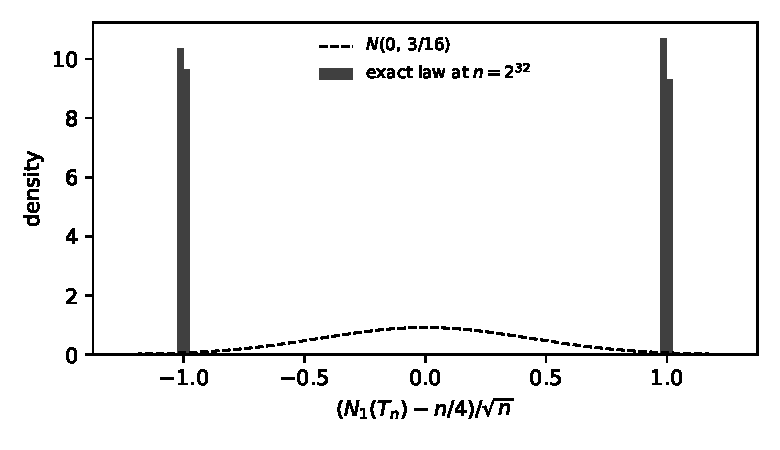
\includegraphics[width=0.75\textwidth]{../figures/thevenin_n2_law.pdf}
\caption{The exact law of $(N_1(T_n)-n/4)/\sqrt n$ at $n=2^{32}$ for the law of \cref{thm:sub}, as a histogram with $100$ bins on $[-1.25,1.25]$, and the density of $\Nor(0,3/16)$ predicted by the conjecture. The two spikes have total mass $0.49996$ and $0.50004$; their standard deviation is $0.0042$.}
\label{fig:law}
\end{figure}

\subsection{The critical law}

At the first stage of the construction of \cref{sec:crit}, $Q^{(0)}$ has three atoms, so the joint law of $(S_N,B_N)$ is explicit: $\Prob(S_N=k,B_N=m)=\binom Nm q^m\binom{N-m}{j}(1/8)^j(5/8)^{N-m-j}$ with $2j=k-m$. With $V_1=1/2$, $\Delta_1=1/2$, $M_1=2$, $v_1=5/32$, $c_1=e^{-16}/\sqrt\pi$ and $\varepsilon_1=1/11$, the displacement is $V_1/(q\Delta_1)=4$, and a floating-point evaluation of the exact formulas gives the following values of the gates.
\[
\begin{array}{c|cc|cc|cc|c}
\log_2n & L_1^- & L_1^+ & \multicolumn{2}{c|}{\text{(G2), rel.\ error}} & \multicolumn{2}{c|}{\text{(G3), }d_K} & \text{(G1)--(G5)}\\
 & & & + & - & + & - \\ \hline
14 & 7679 & 8703 & 0.185 & 0.206 & 0.047 & 0.045 & \text{no}\\
16 & 31743 & 33791 & 0.095 & 0.100 & 0.023 & 0.023 & \text{no}\\
17 & 64087 & 66983 & 0.065 & 0.074 & 0.016 & 0.016 & \text{yes}\\
20 & 520191 & 528383 & 0.024 & 0.025 & 0.006 & 0.006 & \text{yes}
\end{array}
\]
At every size shown, (G1), (G4) and (G5) hold; the accuracy gates (G2) and (G3) are first met at $n=2^{17}$.
So $n_1=2^{17}$, $L_1^\pm=\lfloor 131071/2\pm4\sqrt{131071}\rfloor$, $p_1=2^{-68}$ and $H_1=2^{68}$; the gate (G1) at the second stage then requires $n_2\ge48\cdot2^{68}$, and the later stages grow at least as fast as $n_{r+1}\ge n_r^4$. The construction is explicit but its sizes are far beyond computation after the first stage, which is why the theorem is stated as an existence result.

\section{Remarks}\label{sec:remarks}

The two theorems leave Th\'evenin's theorem and its method intact and identify the missing hypothesis. Writing the outdegrees of $T_n$ as one large coordinate $\Delta$ and $n-1$ small ones, the count $N_1$ is the number of ones among the small coordinates, whose sum is $n-1-\Delta$. Its fluctuations are Gaussian with the conjectured variance when the weight $\mu_\Delta$ of the large coordinate varies slowly across the window $(1-\nu)n\pm C\sqrt n$, so that $\Delta$ absorbs the fluctuations of the sum of the small coordinates; they are not when $\mu$ is lacunary on that window, so that the sum of the small coordinates is pinned to a few values. The argument of \cref{sec:sub} suggests the following form of the conjecture for the subcritical case.

\begin{question}
Let $\mu$ be subcritical with $\mu_0>0$, $\mu_0+\mu_1<1$, finite variance and no exponential moment, and suppose that $\mu_{k+j}/\mu_k\to1$ uniformly in $|j|\le C\sqrt k$ as $k\to\infty$, for every $C>0$; in particular $\mu_k>0$ for all large $k$. Does $(N_A(T_n)-n\mu_A)/\sqrt n$ converge to $\Nor(0,\mu_A(1-\mu_A))$ for every finite $A$?
\end{question}

The regularity in the question holds for $\mu_k\sim ck^{-\beta}$ and more generally for regularly varying tails, and it fails for the laws of this paper. The critical case with infinite variance is more delicate, because the sum of the small coordinates then has non-Gaussian fluctuations of order larger than $\sqrt n$, and \cref{thm:crit} shows that a lacunary tail can again pin that sum; a formulation covering both cases would need to control the local behaviour of $\mu$ at the scale of the fluctuations of the sum.

The examples also bear on Problems 21.2--21.4 of \cite{Janson12}. The second question of Problem 21.2, whether the degree-count central limit theorem extends to critical laws of infinite variance, is answered in the negative by \cref{thm:crit} as far as unrestricted convergence is concerned; its third question, what happens for $0\le\nu<1$, is answered in the same sense by \cref{thm:sub}. The first question concerns the joint convergence and the moment estimates \cite[(21.7)--(21.9)]{Janson12} for critical laws of finite variance without further moment conditions. The joint convergence is proved by Janson \cite[Example 2.2]{Janson16} and is also the case $m=n-1$ of \cref{thm:bb}; the moment estimates are not addressed here. The one-dimensional statement is Kolchin's, with variance $\mu_d(1-\mu_d-(d-1)^2\mu_d/\sigma^2)$. That variance tends to $\mu_d(1-\mu_d)$ as $\sigma^2\to\infty$, which is why the conjecture predicts the latter for infinite variance; for $d=1$ the two agree exactly.

Problem 21.3 asks for the same results for balls in boxes. \Cref{thm:bb} gives the joint central limit theorem when $0<\lambda<\nu$, the case that \cite{Janson12} expects to follow from the methods of \cite{Janson01}, and at $\lambda=\nu$ under a second moment condition, for $m<n\nu$ and for $(m-n\nu)/\sqrt n\to a\in\R$; read for $B_{n-1,n}$, \cref{thm:sub,cor:sub,thm:crit} show that it fails in general when $\lambda>\nu$, and when $\lambda=\nu$ with $\Var(\pi^\rho)=\infty$. Problem 21.4 asks for the same results for the fringe subtree counts of \cite[Theorem 7.12]{Janson12}, the numbers of vertices whose subtree is a given tree. For critical laws of finite variance their joint asymptotic normality is proved by Janson \cite[Corollary 1.8]{Janson16}, with no further moment condition. The number of leaves is the fringe subtree count of the tree with one vertex, so \cref{cor:sub} shows that the extension fails in general for subcritical laws without exponential moment. The critical case with infinite variance is not covered: \cref{thm:crit} concerns $N_1$ only.

Counterexamples of a different kind are known for other tree statistics. Rakotoniaina and Ralaivaosaona \cite{RR} prove asymptotic normality for counts of a fixed tree as a general subtree of a critical conditioned Galton--Watson tree under a moment condition, and give two critical offspring laws violating it for which the variance of the count is no longer of order $n$, so that the fluctuations are not Gaussian at that scale. The failure in \cref{thm:sub,thm:crit} is of a different nature: the centering $n\mu_A$ and the scale $\sqrt n$ of the conjecture are correct, the normalised counts are tight, and the limit along $n_r$ exists and simply is not Gaussian.

\section*{Funding}
The research presented in this paper was supported by the European Research Council (ERC) under the European Union's Horizon Europe research and innovation programme (grant agreement No.~101041711), by the Simons Foundation as part of the Collaboration on the Mathematical and Scientific Foundations of Deep Learning, by Heights Labs, by Convex Nexus Capital, by the Israel Science Foundation (grant number 2258/19), and by the Israel Science Foundation (ISF Grant 4101/25).

\section*{Declaration of competing interest}
The author holds equity in Heights Labs and in Convex Nexus Capital and has a management role at Convex Nexus Capital. These entities are included in the funding declaration above.

\section*{Declaration of generative AI and AI-assisted technologies}
The paper comes out of Math Brain, an ongoing project on the use of AI systems for research mathematics. In September 2026 AI systems (Codex with GPT-6 Astra, OpenAI; Claude Fable 5.1 and Claude Opus 5, Anthropic), working from the conjecture in \cite{Thevenin} and Problem 21.2 of \cite{Janson12}, found the constructions of \cref{thm:sub,thm:crit}, wrote their proofs, the computations of \cref{sec:num} and the Lean file, and searched the literature. In October 2026 Claude Opus 5.5 (Anthropic) proved \cref{lem:llt} in its present generality, \cref{cor:sub} and \cref{thm:bb}, searched the literature on Problems 21.3 and 21.4 of \cite{Janson12}, extended the computations to the number of leaves, and wrote the present text. The arguments have not been refereed by a human mathematician. The author directed the work and is responsible for the content of the paper and for decisions concerning its dissemination.

\section*{Data and code availability}
The code for the exact computations of \cref{sec:num}, the Lean file with its build log and axiom report, and the \LaTeX{} source are available at
\begin{center}
\url{https://github.com/yspennstate/non-gaussian-degree-counts}
\end{center}

\begin{thebibliography}{99}

\bibitem{AD} R. Abraham and J.-F. Delmas, Local limits of conditioned Galton--Watson trees: the condensation case, \emph{Electron. J. Probab.} 19 (2014), no. 56, 1--29.

\bibitem{AL} I. Armend\'ariz and M. Loulakis, Conditional distribution of heavy tailed random variables on large deviations of their sum, \emph{Stochastic Process. Appl.} 121 (2011), 1138--1147.

\bibitem{BLM} S. Boucheron, G. Lugosi and P. Massart, Concentration Inequalities: A Nonasymptotic Theory of Independence, Oxford University Press, 2013.

\bibitem{DM} A. Dvoretzky and Th. Motzkin, A problem of arrangements, \emph{Duke Math. J.} 14 (1947), 305--313.

\bibitem{Janson01} S. Janson, Moment convergence in conditional limit theorems, \emph{J. Appl. Probab.} 38 (2001), 421--437.

\bibitem{Janson12} S. Janson, Simply generated trees, conditioned Galton--Watson trees, random allocations and condensation, \emph{Probab. Surv.} 9 (2012), 103--252.

\bibitem{Janson16} S. Janson, Asymptotic normality of fringe subtrees and additive functionals in conditioned Galton--Watson trees, \emph{Random Structures Algorithms} 48 (2016), 57--101.

\bibitem{JS} T. Jonsson and S. \"O. Stef\'ansson, Condensation in nongeneric trees, \emph{J. Stat. Phys.} 142 (2011), 277--313.

\bibitem{Kolchin} V. F. Kolchin, Random Mappings, Optimization Software, New York, 1986.

\bibitem{Kortchemski} I. Kortchemski, Limit theorems for conditioned non-generic Galton--Watson trees, \emph{Ann. Inst. Henri Poincar\'e Probab. Stat.} 51 (2015), 489--511.

\bibitem{Pitman} J. Pitman, Combinatorial Stochastic Processes, Lecture Notes in Mathematics 1875, Springer, 2006.

\bibitem{RR} F. Rakotoniaina and D. Ralaivaosaona, Asymptotic normality for general subtree counts in conditioned Galton--Watson trees, arXiv:2603.08076 (2026).

\bibitem{Thevenin} P. Th\'evenin, Vertices with fixed outdegrees in large Galton--Watson trees, \emph{Electron. J. Probab.} 25 (2020), paper no. 64, 25 pp.; arXiv:1812.07365.

\end{thebibliography}

\end{document}
